\subsection{Schnittstellenbeschreibung}
\subsubsection{Spezifikation BluetoothController-Klasse}

\lstsettingjava

\begin{table}[h!]
\begin{tabular}{|l|l|l|l|l|}
\hline 
Version & Datum & Autor & Bemerkung & Status \\ 
\hline 
1.0.0 & 26.03.2015 & SN & Initiale Fassung & freigegeben \\ 
\hline 
1.0.1 & 15.04.2015 & SN & Initiale Fassung & freigegeben \\ 
\hline 
\end{tabular} 
\caption{Steckbrief der Klasse BluetoothController}
\end{table}

\textbf{Operationen und Datenstukturen}
 
Die Schnittstelle stellt folgende Methoden und Datentypen zur Verfügung:  \\
\begin{figure}[h!]          
	\centering             
	%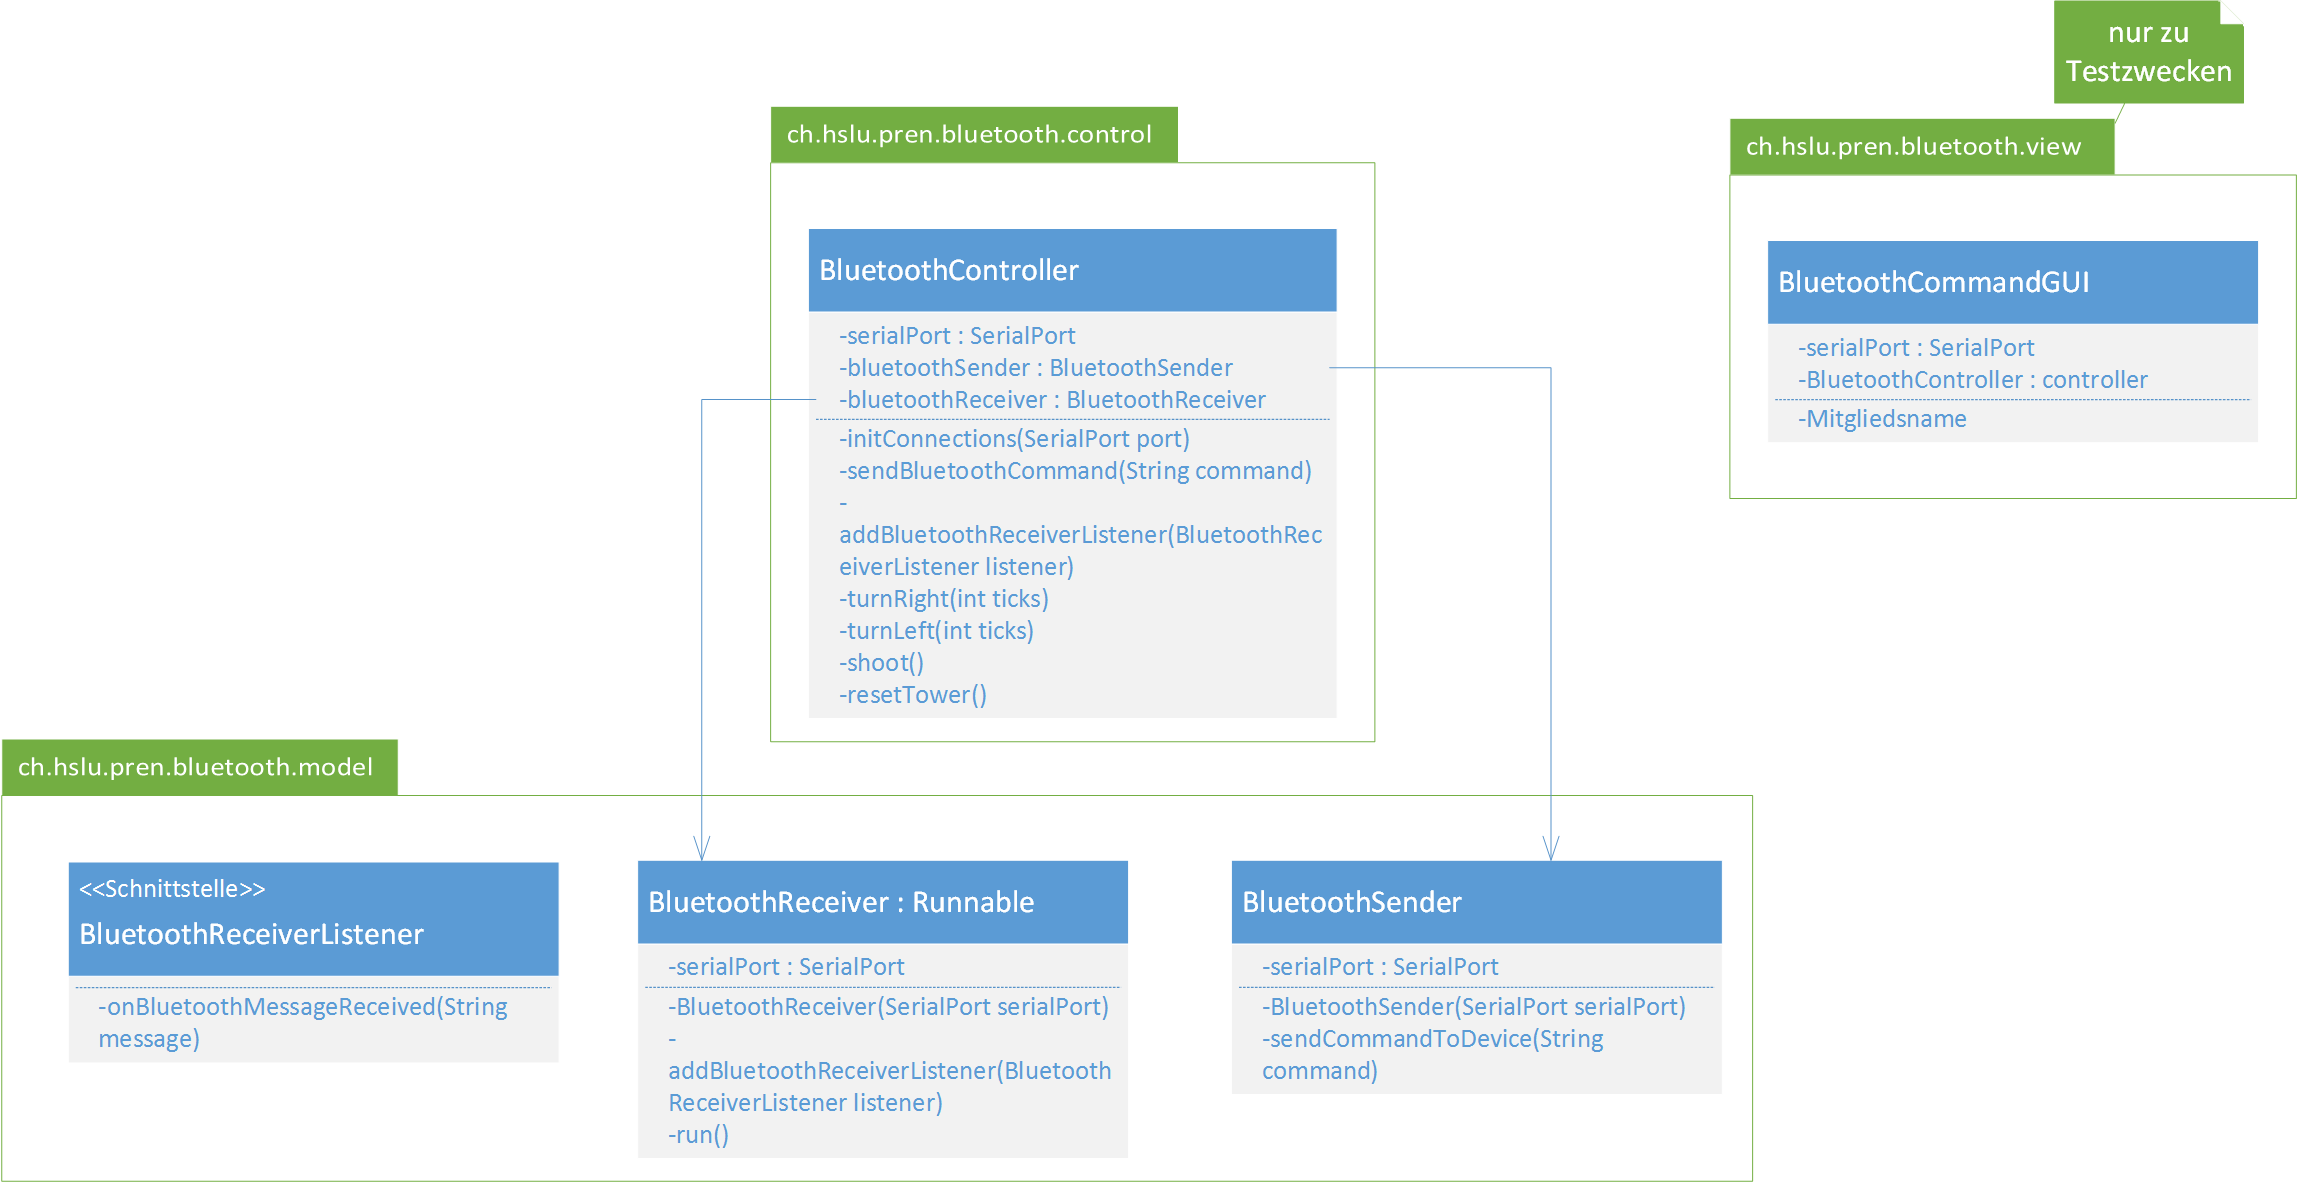
\includegraphics[width=1\textwidth]{../fig/Klassendiagramm Bluetoothmodul.png}
	\caption{Klassendiagramm Bluetoothmodul}
	\label{fig:Klassendiagramm Bluetoothmodul}        
\end{figure} \\
Details zu den Methoden und den verwendeten Datentypen sind in der JavaDoc festgehalten. \\
\textbf{Einsatz, Abläufe, Voraussetzungen und Zusicherungen}\\
\begin{itemize}
	\item{Bevor Daten über die Schnittstelle ausgetauscht werden können, muss mittels initConnections(String serialPortName) ein gültiger serieller Port definiert werden. Der konfigurierte Port gilt für alle darauf folgenden command-Aufrufe. }
	\item{Ein Wechsel des seriellen Ports, d.h. Umkonfigurierung mit initConnections(String serialPortName), ist nun jederzeit möglich.}
	\item{Eine Klasse, die das Interface BluetoothReceiverListener implementiert, kann als Observer für empfangene Nachrichten des BluetoothReceivers fungieren.}
\end{itemize}
\textbf{Aufbau und Konfiguration} \\
Keine zusätzlichen Informationen. \\
\textbf{Fehlerbehandlung}\\
Die Fehlerbehandlung wird über unchecked Exceptions realisiert. Details siehe JavaDoc. \\
\textbf{Beispielverwendung}\\
Der folgende Codeausschnitt zeigt die Verwendung der Schnittstelle anhand einer beispielhaften Implementation BluetoothController: \\
\lstinputlisting{../../sw/PrenManager/src/TestGUI/newClass.java}

